\documentclass[11pt,a4paper]{article}

\usepackage[T1]{fontenc}
\usepackage[utf8]{inputenc}
\usepackage{lmodern}
\usepackage{mathptmx}
\usepackage[Symbol]{upgreek}
\usepackage[margin=1.5cm,top=1.0cm,bottom=1.0cm]{geometry}
\usepackage{microtype}
\usepackage{multicol}
\usepackage{amsmath}
\usepackage{graphicx}
\usepackage[font=footnotesize,labelfont=bf,skip=2pt]{caption}
\usepackage[hidelinks]{hyperref}

\pagestyle{empty}
\setlength{\parindent}{0pt}
\setlength{\parskip}{3pt}
\linespread{1.0}
\setlength{\abovedisplayskip}{2pt}
\setlength{\belowdisplayskip}{2pt}
\setlength{\intextsep}{2pt}

% Every number below is generated from the result files, never typed by hand.
% Auto-generated by make_paper_assets.py -- do not edit by hand.
\newcommand{\bestLeakDeadPct}{96}
\newcommand{\bestLeakLambda}{10}
\newcommand{\bestLeakMode}{mean}
\newcommand{\bestLeakRouting}{0.0003}
\newcommand{\bestLeakValue}{0.0020}
\newcommand{\bestRoutAlivePct}{83}
\newcommand{\bestRoutLeak}{0.296}
\newcommand{\bestRoutValue}{0.40}
\newcommand{\blockOffPositive}{4}
\newcommand{\blockPositive}{19}
\newcommand{\blockRuns}{5}
\newcommand{\blockSig}{10}
\newcommand{\blockSigHolm}{1}
\newcommand{\blockSigTauFifty}{1}
\newcommand{\blockSigTauFive}{3}
\newcommand{\blockSigTauTen}{4}
\newcommand{\blockSigTauTwenty}{2}
\newcommand{\blockSignP}{2.0\times10^{-5}}
\newcommand{\blockTotal}{20}
\newcommand{\budget}{10}
\newcommand{\cgGptSent}{+0.109}
\newcommand{\cgGptTox}{+0.133}
\newcommand{\cgPGptSent}{$<$0.001}
\newcommand{\cgPGptTox}{0.879}
\newcommand{\cgPQwenSent}{0.004}
\newcommand{\cgPQwenTox}{0.007}
\newcommand{\cgQwenSent}{+0.277}
\newcommand{\cgQwenTox}{+0.127}
\newcommand{\contrastFVUlamOne}{0.250}
\newcommand{\contrastFVUlamTen}{1.03}
\newcommand{\contrastRoutLamOne}{0.36}
\newcommand{\degenCorrMax}{-0.28}
\newcommand{\dimGptSent}{+0.404}
\newcommand{\dimGptTox}{+0.130}
\newcommand{\dimQwenSent}{+0.413}
\newcommand{\dimQwenTox}{+0.044}
\newcommand{\dimSentSAEbetter}{0}
\newcommand{\dimSentSAEworse}{12}
\newcommand{\dimSentTotal}{12}
\newcommand{\dimToxSAEbetter}{3}
\newcommand{\dimToxSAEworse}{0}
\newcommand{\dimToxTotal}{8}
\newcommand{\dissBUnw}{-0.447}
\newcommand{\dissBWan}{+0.184}
\newcommand{\dissGUnw}{+0.183}
\newcommand{\dissGWan}{-0.411}
\newcommand{\dissRUnw}{-0.039}
\newcommand{\dissRWan}{+0.001}
\newcommand{\evVanGPT}{80}
\newcommand{\evVanQwen}{96}
\newcommand{\fvuCGGPT}{0.277}
\newcommand{\fvuCGQwen}{0.066}
\newcommand{\fvuVanGPT}{0.203}
\newcommand{\fvuVanQwen}{0.045}
\newcommand{\layerDisagree}{4}
\newcommand{\layerFracMax}{85}
\newcommand{\layerFracMin}{27}
\newcommand{\layerGptAUC}{0.816}
\newcommand{\layerGptLoss}{45}
\newcommand{\layerGptProbe}{11}
\newcommand{\layerGptSteer}{7}
\newcommand{\layerScans}{4}
\newcommand{\leakRatioBestVsRout}{146}
\newcommand{\leakRoutingCorr}{+0.03}
\newcommand{\nPrimaryRuns}{5}
\newcommand{\nRuns}{6}
\newcommand{\nSynthSeeds}{20}
\newcommand{\penformConfigs}{12}
\newcommand{\penformSeeds}{2}
\newcommand{\qtoxLfifteenEff}{+0.062}
\newcommand{\qtoxLfifteenPPL}{37.6}
\newcommand{\qtoxLtenEff}{+0.056}
\newcommand{\qtoxLtenPPL}{6.5}
\newcommand{\scarGptSent}{+0.118}
\newcommand{\scarGptTox}{+0.194}
\newcommand{\scarPGptSent}{$<$0.001}
\newcommand{\scarPGptTox}{0.022}
\newcommand{\scarPQwenSent}{$<$0.001}
\newcommand{\scarPQwenTox}{0.075}
\newcommand{\scarQwenSent}{+0.147}
\newcommand{\scarQwenTox}{+0.075}
\newcommand{\specMax}{16.6}
\newcommand{\specMaxBuf}{4.33}
\newcommand{\specMaxLamFive}{14.0}
\newcommand{\specNoBufLamFive}{0.91}
\newcommand{\specNoBufLamOne}{1.5}
\newcommand{\specOffMax}{1.65}
\newcommand{\specOffMin}{0.99}
\newcommand{\sqFVUspread}{1.2\times10^{-4}}
\newcommand{\sqLeakLamThirty}{0.435}
\newcommand{\sqLeakLamZero}{0.495}
\newcommand{\sqPenShare}{0.5}
\newcommand{\sqPenTermThirty}{8.7\times10^{-4}}
\newcommand{\sqRoutMax}{0.012}
\newcommand{\synthBAliveMin}{100}
\newcommand{\synthRouting}{0.35}
\newcommand{\synthRoutingOff}{0.010}
\newcommand{\vanFVUpenform}{0.173}
\newcommand{\vsSSVgptPmax}{0.40}
\newcommand{\vsSSVgptPmin}{0.24}
\newcommand{\vsSSVgptPositive}{3}
\newcommand{\vsSSVgptSig}{0}
\newcommand{\vsSSVgptTotal}{4}
\newcommand{\vsSSVqwenPositive}{8}
\newcommand{\vsSSVqwenPrimSig}{4}
\newcommand{\vsSSVqwenPrimTotal}{6}
\newcommand{\vsSSVqwenSig}{6}
\newcommand{\vsSSVqwenSigHolm}{3}
\newcommand{\vsSSVqwenTotal}{8}
\newcommand{\vsScarQwenSig}{1}
\newcommand{\vsScarSig}{1}
\newcommand{\vsScarTotal}{12}

% Auto-generated by make_ea_assets.py -- do not edit by hand.
\newcommand{\ghBadGen}{+0.111}
\newcommand{\ghBadNeg}{+30.1}
\newcommand{\ghBadNegHi}{+31.7}
\newcommand{\ghBadNegLo}{+28.4}
\newcommand{\ghBadPos}{+9.1}
\newcommand{\ghGoodGen}{+0.092}
\newcommand{\ghGoodNeg}{+6.7}
\newcommand{\ghGoodNegHi}{+7.2}
\newcommand{\ghGoodNegLo}{+6.5}
\newcommand{\ghGoodPos}{+26.6}
\newcommand{\ghRandGen}{+0.078}
\newcommand{\ghRandNeg}{+9.7}
\newcommand{\ghRandNegHi}{+14.6}
\newcommand{\ghRandNegLo}{+6.6}
\newcommand{\ghRandPos}{+11.1}
\newcommand{\ghRelearnBad}{0.54}
\newcommand{\ghRelearnRand}{0.52}
\newcommand{\ghRouting}{0.37}
\newcommand{\ghSeeds}{3}
\newcommand{\ghWikiBucket}{120}
\newcommand{\ghWikiCostPct}{105}
\newcommand{\ghWikiPlain}{59}
\newcommand{\glBadGen}{-0.028}
\newcommand{\glBadNeg}{+9.0}
\newcommand{\glBadNegHi}{+9.0}
\newcommand{\glBadNegLo}{+9.0}
\newcommand{\glBadPos}{+8.6}
\newcommand{\glGoodGen}{-0.055}
\newcommand{\glGoodNeg}{+8.3}
\newcommand{\glGoodNegHi}{+8.3}
\newcommand{\glGoodNegLo}{+8.2}
\newcommand{\glGoodPos}{+8.1}
\newcommand{\glRandGen}{+0.022}
\newcommand{\glRandNeg}{+9.3}
\newcommand{\glRandNegHi}{+10.6}
\newcommand{\glRandNegLo}{+8.0}
\newcommand{\glRandPos}{+9.1}
\newcommand{\glRelearnBad}{0.67}
\newcommand{\glRelearnRand}{0.68}
\newcommand{\glRouting}{0.00}
\newcommand{\glSeeds}{3}
\newcommand{\glWikiBucket}{59}
\newcommand{\glWikiPlain}{59}
\newcommand{\gtBadGen}{+0.048}
\newcommand{\gtBadNeg}{+26.5}
\newcommand{\gtBadNegHi}{+29.2}
\newcommand{\gtBadNegLo}{+24.8}
\newcommand{\gtBadPos}{+9.6}
\newcommand{\gtGoodGen}{+0.080}
\newcommand{\gtGoodNeg}{+7.7}
\newcommand{\gtGoodNegHi}{+7.9}
\newcommand{\gtGoodNegLo}{+7.6}
\newcommand{\gtGoodPos}{+21.6}
\newcommand{\gtRandGen}{+0.085}
\newcommand{\gtRandNeg}{+10.5}
\newcommand{\gtRandNegHi}{+13.0}
\newcommand{\gtRandNegLo}{+7.5}
\newcommand{\gtRandPos}{+12.2}
\newcommand{\gtRelearnBad}{0.63}
\newcommand{\gtRelearnRand}{0.63}
\newcommand{\gtRouting}{0.29}
\newcommand{\gtSeeds}{3}
\newcommand{\gtWikiBucket}{69}
\newcommand{\gtWikiCostPct}{19}
\newcommand{\gtWikiPlain}{58}
\newcommand{\slBadGen}{-0.011}
\newcommand{\slBadNeg}{+19.7}
\newcommand{\slBadNegHi}{+21.2}
\newcommand{\slBadNegLo}{+18.3}
\newcommand{\slBadPos}{+7.3}
\newcommand{\slGoodGen}{-0.040}
\newcommand{\slGoodNeg}{+6.9}
\newcommand{\slGoodNegHi}{+9.2}
\newcommand{\slGoodNegLo}{+4.5}
\newcommand{\slGoodPos}{+26.3}
\newcommand{\slRandGen}{+0.001}
\newcommand{\slRandNeg}{+0.2}
\newcommand{\slRandNegHi}{+0.3}
\newcommand{\slRandNegLo}{+0.1}
\newcommand{\slRandPos}{+0.1}
\newcommand{\slRelearnBad}{0.74}
\newcommand{\slRelearnRand}{0.74}
\newcommand{\slRouting}{0.87}
\newcommand{\slSeeds}{2}
\newcommand{\slWikiBucket}{1932}
\newcommand{\slWikiPlain}{1957}
\newcommand{\ssBadGen}{-0.116}
\newcommand{\ssBadNeg}{+3.9}
\newcommand{\ssBadNegHi}{+4.6}
\newcommand{\ssBadNegLo}{+3.2}
\newcommand{\ssBadPos}{-0.4}
\newcommand{\ssGoodGen}{+0.064}
\newcommand{\ssGoodNeg}{-0.3}
\newcommand{\ssGoodNegHi}{+0.1}
\newcommand{\ssGoodNegLo}{-0.8}
\newcommand{\ssGoodPos}{+3.4}
\newcommand{\ssRandGen}{-0.020}
\newcommand{\ssRandNeg}{+0.5}
\newcommand{\ssRandNegHi}{+0.5}
\newcommand{\ssRandNegLo}{+0.4}
\newcommand{\ssRandPos}{+0.4}
\newcommand{\ssRelearnBad}{0.67}
\newcommand{\ssRelearnRand}{0.62}
\newcommand{\ssRouting}{0.92}
\newcommand{\ssSeeds}{2}
\newcommand{\ssWikiBucket}{7208}
\newcommand{\ssWikiPlain}{12579}


% \bstctlcite normally comes from the IEEEtran class; defined here so IEEEtran.bst can read its
% control entry (at most three authors, otherwise "et al.") under the article class.
\makeatletter
\def\bstctlcite{\@ifnextchar[{\@bstctlcite}{\@bstctlcite[@auxout]}}
\def\@bstctlcite[#1]#2{\@bsphack
  \@for\@citeb:=#2\do{%
    \edef\@citeb{\expandafter\@firstofone\@citeb}%
    \if@filesw\immediate\write\csname #1\endcsname{\string\citation{\@citeb}}\fi}%
  \@esphack}
\makeatother

\newcommand{\Wb}{\mathrm{W}}
\newcommand{\Nb}{\mathrm{N}}
\newcommand{\Ub}{\mathrm{U}}
\newcommand{\avg}{\operatorname{mean}}
\newcommand{\hd}[1]{\textbf{#1}\enspace}

\begin{document}
\bstctlcite{IEEEexample:BSTcontrol}

\begin{center}
{\large\bfseries Localising Unwanted Knowledge in Language Models\\[1pt] with Reserved Buckets and a Neutral Buffer}\\[4pt]
Varanasi Sathveek, Vanamala Aravind, Pula Naga Manikanta, K.\ Hima Bindu\\
{\small Department of Computer Science \& Engineering, National Institute of Technology Andhra Pradesh, India\\
Extended abstract \,\textbullet\, CARE 2026 \,\textbullet\, Track: Social Impact of AI}
\end{center}

\hd{Objective.}
Removing a harmful behaviour from a language model without damaging everything else is hard,
because models store far more concepts than they have neurons and the concepts overlap
(superposition)~\cite{elhage2022toy}. Steering finds a direction after
training~\cite{turner2023actadd,rimsky2024caa,li2023iti}, sparse-autoencoder (SAE) methods tie a
behaviour to one unit~\cite{harle2024scar} or search for units afterwards~\cite{he2025saessv}, and
gradient routing masks gradients to localise a capability~\cite{cloud2024gradient}; none gives features
shared by opposing behaviours a place of their own. The obvious penalty can also be met by silencing
units, which the usual \emph{leakage} measure misses ($r=\leakRoutingCorr$ with actual routing). Our
objective is to reserve, before training, a fixed place for one unwanted behaviour, such as toxic
language or negative sentiment, so it can later be cut out without touching the rest.

\hd{Keywords:} mechanistic interpretability; sparse autoencoders; superposition; model editing;
knowledge removal

\hd{Method.}
Take a layer with $m$ hidden units: the MLP neurons of a language model, or the
dictionary units of an SAE. We set aside $\lfloor\uptau m\rfloor$ of them as a wanted bucket $\Wb$
and as many as an unwanted bucket $\Ub$, where $0<\uptau\le\frac12$ is the fraction per bucket (we
tried 0.05 to 0.5; at $\frac12$ no buffer is left). The remaining units
form a \emph{neutral buffer} $\Nb$ that is never penalised, so features shared by both behaviours
have somewhere to go. With $s_S$ the share of activity falling in bucket
$S$ and $y$ the label of the training text ($y=0$ unwanted), we train with
$L=L_{\mathrm{task}}+\uplambda P$, where
\begin{equation}
  P=-\tfrac12\Big[\big(\avg_{y=0}s_{\Ub}-\avg_{y=1}s_{\Ub}\big)+\big(\avg_{y=1}s_{\Wb}-\avg_{y=0}s_{\Wb}\big)\Big].
\end{equation}
This rewards $\Ub$ for \emph{carrying} unwanted activity rather than staying silent. Afterwards $\Ub$
is deleted: inside a model we zero its neurons' weights; in an SAE we scale its units down and add
only the resulting change to the frozen model.

\hd{Experiments.}
We test the idea at three scales, always comparing the deletion of $\Ub$ with
deleting a random bucket of the same size. First, a toy classifier on two overlapping Gaussian
classes (\nSynthSeeds{} seeds). Second, buckets inside
GPT-2's MLP neurons (layers 5--9, $\uptau=0.1$) during fine-tuning, and inside a small GPT-style
model trained from scratch. The data are IMDB reviews with negative sentiment as the unwanted
behaviour; we measure perplexity on held-out negative and positive reviews, and on WikiText-103
for general fluency. Third, buckets inside SAEs~\cite{gao2024scaling} on frozen GPT-2 and
Qwen2.5-1.5B for sentiment (IMDB) and toxicity (RealToxicityPrompts), against a normal SAE, a single
conditioned unit and difference-in-means steering at equal sparsity, edit size and fluency cost
(2--3 seeds each).

\hd{Results.}
\emph{Toy:} we define specificity $S$ as the drop in the classifier's AUC at recognising the
unwanted class when $\Ub$ is deleted, divided by the same drop when a random bucket is deleted
($S=1$ is chance). With a wide buffer ($\uptau=0.1$) $S$ reaches \specMax; with no buffer
($\uptau=\frac12$) it falls to \specNoBufLamOne{} at $\uplambda=1$ and to \specNoBufLamFive{} at
$\uplambda=5$. \emph{Inside GPT-2} ($\uplambda=3$): deleting
$\Ub$ raises perplexity on negative reviews by \gtBadNeg\% but on positive reviews by only \gtBadPos\%
in all \gtSeeds{} runs, deleting $\Wb$ does the reverse, and a random bucket hurts both equally
(Fig.~1), at a \gtWikiCostPct\% cost in general fluency. The model trained from scratch shows the
same pattern. \emph{SAEs:} removing $\Ub$ beats removing a random bucket in \blockPositive{} of
\blockTotal{} settings ($p=\blockSignP$); a bucketed SAE beats a normal SAE on Qwen
(\vsSSVqwenSig{}/\vsSSVqwenTotal{} tests) but not on GPT-2 (\vsSSVgptSig{}/\vsSSVgptTotal); difference-in-means
steering wins on sentiment, while SAEs win on toxicity. \emph{Ablations, errors and generality:}
the pattern needs both the buffer and a strong enough penalty ($\uplambda=1$ forms no buckets,
$\uplambda=10$ costs \ghWikiCostPct\% in fluency) and holds across two models, two concepts, and both
fine-tuning and training from scratch; however, deleting $\Ub$ did not reliably make the model
\emph{write} less negatively, and the knowledge can be relearned.

\begin{figure}[h]
  \centering
  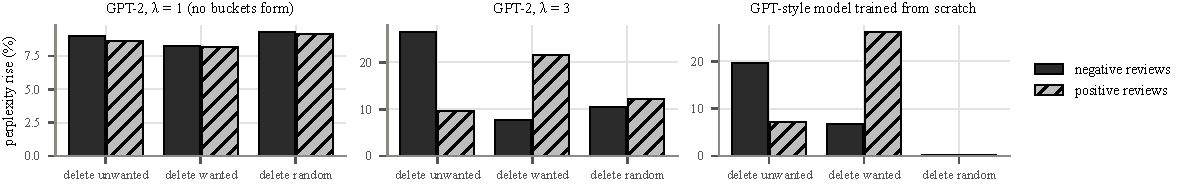
\includegraphics[width=0.66\linewidth]{figures/fig_inmodel_compact.pdf}
  \caption{Perplexity rise on held-out reviews after deleting a bucket. Once buckets form, deleting
  $\Ub$ mainly hurts negative reviews.}
\end{figure}

\hd{Inference.}
The knowledge behind an unwanted behaviour can be placed in a chosen location and removed
selectively, as measured by perplexity, and the neutral buffer is what makes this work. Knowledge moves more reliably than behaviour; closing
that gap is our next step. Leakage alone should not be used to judge such methods.

\hd{References}
{\scriptsize
\renewcommand{\section}[2]{}%
\makeatletter
\renewcommand\@openbib@code{\setlength\itemsep{0pt}\setlength\parsep{0pt}\setlength\topsep{0pt}}%
\makeatother
\setlength{\parskip}{0pt}\linespread{1.0}\selectfont
\setlength{\columnsep}{14pt}\setlength{\multicolsep}{2pt}
\begin{multicols}{2}
\bibliographystyle{IEEEtran}
\bibliography{IEEEabrv,references}
\end{multicols}}

\end{document}
